\chapter{简支梁平面问题的解析解}
\setlength{\footskip}{15.61334pt}
\label{cha:Analyticalsolution}
本章节主要讨论《工程弹塑性力学引论》例~B.2~中简支梁平面问题\cite{gctsxyl}的解析解,通过半逆解法来求解简支梁的应力、应变、位移场量\cite{LXYS201201011,SCJI202306051},并对结果进行分析和可视化。
\section{平面问题描述}
所求解的简支梁如图\ref{fig:load}所示,长度为~$l$,截面宽度为单位~1,截面高度为~$h$。梁的上边缘受均布荷载~$q$~作用。在梁的质心处建立直角坐标系,沿长度方向为~$x$~轴,沿高度方向为~$y$~轴。考虑到该简支梁的截面高度远大于宽度,在求解时可以认为该问题是平面应力问题,因此解析解与~$z$~方向无关。
\begin{figure}[htbp]
    \centering
	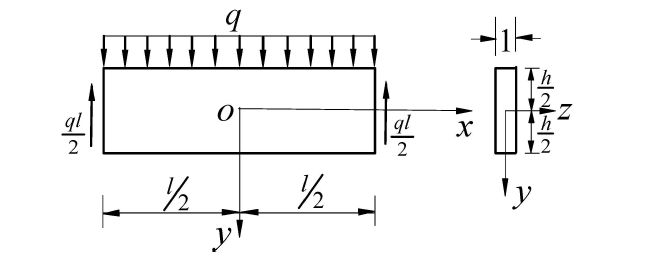
\includegraphics[width=0.7\textwidth]{figure1}
    \caption{简支梁承受均布荷载}
    \label{fig:load}
\end{figure}
\section{半逆解法求解}
\subsection{公式推导}
弹性力学的平面问题可以归结为以下三组方程:\\
1)平衡方程
\begin{equation}\label{eq1}
    \left\{
        \begin{array}{l}
            \dfrac{\partial \sigma_x}{\partial x} + \dfrac{\partial \tau_{xy}}{\partial y} + f_x = 0\\
            \dfrac{\partial \tau_{yx}}{\partial x} + \dfrac{\partial \sigma_y}{\partial y} + f_y = 0
        \end{array}
    \right.
\end{equation} 
2)协调方程
\begin{equation}\label{eq2}
    \frac{\partial^2 \varepsilon_x}{\partial x^2} +\frac{\partial^2 \varepsilon_y}{\partial y^2} = 2\frac{\partial^2 \varepsilon_{xy}}{\partial x \partial y}
\end{equation} 
3)应力-应变关系
\begin{equation}\label{eq3}
    \left\{
        \begin{array}{l}
            \varepsilon_x = \dfrac{1}{E}(\sigma_x-\nu \sigma_y)\vspace{1ex}\\
            \varepsilon_y = \dfrac{1}{E}(\sigma_y-\nu \sigma_x)\vspace{1ex}\\
            \varepsilon_{xy} = \dfrac{1}{2G}\tau_{xy}
        \end{array}
    \right.
\end{equation} 

将应力-应变关系\eqref{eq3}和平衡方程\eqref{eq1}代入协调方程\eqref{eq2},且不考虑体力,可化简得到:
\begin{equation}\label{eq4}
    \bigtriangledown^2(\sigma_x+\sigma_y) = 0
\end{equation} 

再考虑无体力的平衡方程:
\begin{equation}\label{eq5}
    \left\{
        \begin{array}{l}
            \dfrac{\partial \sigma_x}{\partial x} + \dfrac{\partial \tau_{xy}}{\partial y} = 0\vspace{1ex}\\
            \dfrac{\partial \tau_{yx}}{\partial x} + \dfrac{\partial \sigma_y}{\partial y} = 0
        \end{array}
    \right.
\end{equation} 
结合格林(Green)定理,可知存在势函数~$P$~和~$Q$,满足:
\begin{equation}\label{eq6}
    \sigma_x = \frac{\partial P}{\partial y}~,~\tau_{xy} = -\frac{\partial P}{\partial x}~,~\sigma_y = \frac{\partial Q}{\partial x}~,~\tau_{yx} = -\frac{\partial Q}{\partial y}
\end{equation}  

进一步结合剪应力互等定理,剪力满足:
\begin{equation}\label{eq7}
    \tau_{xy}-\tau_{yx} = \frac{\partial Q}{\partial y}-\frac{\partial P}{\partial x}=0
\end{equation}  
同样可以使用格林定理得到势函数~$\phi$,满足:
\begin{equation}\label{eq8}
    P = \frac{\partial \phi}{\partial y}~,~Q = \frac{\partial \phi}{\partial x}
\end{equation}  
其中~$\phi$~为艾里(Airy)应力函数。将~$P$、~$Q$~代入式\eqref{eq6},可得应力分量方程:
\begin{equation}\label{eq9}
    \sigma_x = \frac{\partial^2 \phi}{\partial y^2}~,~\sigma_y = \frac{\partial^2 \phi}{\partial x^2}~,~\tau_{xy} = -\frac{\partial^2 \phi}{\partial x \partial y}
\end{equation} 
再将\eqref{eq9}带入简化后的无体力协调方程\eqref{eq4},整理可得应力函数方程:
\begin{equation}\label{eq10}
    \bigtriangledown^2\bigtriangledown^2 \phi = 0
\end{equation}
其中~$\bigtriangledown^2\bigtriangledown^2$~被称为双调和算符。

在半逆解法中,应力函数的构成可以考虑微分方程解法中的分离变量法,假定应力函数的形式为:
\begin{equation}\label{eq11}
    \phi = g(x)f(y)
\end{equation}
带入双调和方程\eqref{eq10},有:
\begin{equation}\label{eq12}
    \bigtriangledown^2\bigtriangledown^2 \phi = g''''(x)f(y)+2g''(x)f''(y)+g(x)f''''(y) = 0
\end{equation}
若考虑函数~$g(x)$~为多项式形式,将多项式带入式\eqref{eq12},可得关于~$f(y)$、$f^{''}(y)$、$f^{''''}(y)$~构成系数的多项式方程。该方程恒等于~0~的条件是系数恒等于~0。由此可建立~$f(y)$~的微分方程,进而求出~$f(y)$~的表达式。若应力函数是\eqref{eq11}的线性组合,即:
\begin{equation}\label{eq13}
    \phi = \sum_{i} g_i(x)f_i(y)
\end{equation}
仍可以用上述过程求解。
\subsection{问题求解}
首先对问题进行简单的分析,$\sigma_x$~主要是由弯矩引起,$\sigma_y$~主要是由~$q$~引起(挤压应力),$\tau_{xy}$~主要是由剪力引起。又因为~$q$~恒定不变,且结构在图示坐标系下对称,因此假定~$\sigma_y$~与~$x$~无关,推得:
\begin{equation}\label{eq14}
    \sigma_y = \frac{\partial^2 \phi}{\partial x^2} = f(y)
\end{equation}
对上式积分,可得应力函数~$\phi$~的基本表达式为:
\begin{equation}\label{eq15}
    \phi = \frac{1}{2}x^2f(y)+xf_1(y)+f_2(y)
\end{equation}
其中~$f(y)$、~$f_1(y)$、$f_2(y)$~为任意待定的多项式函数。
进一步通过式\eqref{eq9}求得其中~$\tau_{xy}$~的表达式为:
\begin{equation}\label{eq16}
    \tau_{xy} = -\frac{\partial^2 \phi}{\partial x \partial y} = -xf'(y)+f_1'(y)
\end{equation}

接着观察到剪应力~$\tau_{xy}$~关于~y~轴反对称,是关于~x~的奇函数,因此上式中的~$f_1'(y)$~恒等于~0,从而推得:
\begin{equation}\label{eq17}
    \tau_{xy} = -xf'(y)
\end{equation}
对~$\tau_{xy}$~积分,反推得应力函数~$\phi$~修正表达式为:
\begin{equation}\label{eq18}
    \phi = \frac{1}{2}x^2f(y)+f_2(y)
\end{equation}  

将修正的表达式代入式\eqref{eq12},可得:
\begin{equation}\label{eq19}
    \frac{1}{2}x^2f''''(y)+ 2f''(y)+f_2''''(y) = 0
\end{equation}  
该关于x的系数方程恒成立的条件为系数恒等于~0,即:
\begin{equation}\label{eq20}
    \left\{
        \begin{array}{l}
            \dfrac{1}{2}f''''(y) = 0 \\
            2f''(y)+f_2''''(y) = 0
        \end{array}
    \right.
\end{equation} 
利用多次不定积分,可得上述微分方程组的解如下:
\begin{equation}\label{eq21}
    \left\{
        \begin{array}{l}
            f(y) = \text{A}+\text{B}y+\text{C}y^2+\text{D}y^3 \\
            f_2(y) = \text{E}+\text{F}y+\text{G}y^2+\text{H}y^3-\dfrac{1}{6}\text{C}y^4-\dfrac{1}{10}\text{D}y^5
        \end{array}
    \right.
\end{equation}
其中,A$\sim$H~均为待定系数;将上式代入式\eqref{eq18}后,再将得出的~$\phi$~回代入式\eqref{eq9},可得应力函数的表达式为:
\begin{equation}\label{eq22}
    \left\{
        \begin{array}{l}
            \sigma_x = \dfrac{1}{2}x^2f''(y)+f''_2(y) = \dfrac{1}{2}x^2(2\text{C}+6\text{D}y)+2\text{G}+6\text{H}y-2\text{C}y^3-2\text{D}y^4\\
            \sigma_y = f(y) = \text{A}+\text{B}y+\text{C}y^2+\text{D}y^3\\
            \tau_{xy} = -xf'(y) = -x(\text{B}+2\text{C}y+3\text{D}y^2)
        \end{array}
    \right.
\end{equation}

为了求解应力函数中的待定系数,需要利用该问题的边界条件。对于基于应力求解,用位移边界条件还需积分,较难处理,故一般都化为力边界条件代入。上下两个边界为主要边界,应该严格满足边界条件,左右两个次要边界可以用圣维南原理不严格满足,其中:\\
1)主要边界条件(上下两侧的应力)
\begin{subequations}\label{eq23}
    \begin{numcases} 
         ~~\sigma_y = 0, &\mbox{y = $\dfrac{1}{2}h$}\label{eq23a}  \\
         ~\sigma_y = -q, &\mbox{y = $-\dfrac{1}{2}h$}\label{eq23b} \\
         ~\tau_{xy} = 0, &\mbox{y = $\pm$ $\dfrac{1}{2}h$}\label{eq23c}
    \end{numcases}
\end{subequations}
2)次要边界条件(左右两端的轴力、剪力、弯矩)
\begin{subequations}\label{eq24} 
    \begin{numcases}  
         ~~\int_{-h/2}^{h/2}\sigma_x dy = 0, &\mbox{x = $\pm$ $\dfrac{1}{2}l$}\label{eq24a} \\
         ~\int_{-h/2}^{h/2}\tau_{xy} dy = -\frac{1}{2}ql, &\mbox{x = $\pm$ $\dfrac{1}{2}l$}\label{eq24b}\\
         ~\int_{-h/2}^{h/2}\sigma_xy dy = 0, &\mbox{x = $\pm$ $\dfrac{1}{2}l$}\label{eq24c}
    \end{numcases}
\end{subequations}
由式\eqref{eq23c}计算可得待定系数~C~=~0,B~=~$-\dfrac{3}{4}Dh^2$。将计算所得的系数值继续代入式\eqref{eq23a}和\eqref{eq23b},计算可得系数A~=~$-\dfrac{1}{2}q$,B~=~$\dfrac{3}{2h}q$,D~=~$-\dfrac{2}{h^3}q$。继续将已知的所有系数值代入式\eqref{eq24a}和\eqref{eq23c},计算可得系数~G~=~0,H~=~$\dfrac{1}{4h^3}ql^2-\dfrac{1}{10h}q$。

将所求的全部系数值代入式\eqref{eq22},可得最终的应力函数表达式:
\begin{equation}\label{eq25}
    \left\{
        \begin{array}{l}
            \sigma_x = -\dfrac{6q}{h^3}x^2y+\dfrac{4q}{h^3}y^3+(\dfrac{3ql^2}{2h^3}-\dfrac{3q}{5h})y \vspace{1ex}\\
            \sigma_y = -\dfrac{2q}{h^3}y^3+\dfrac{3q}{2h}y-\dfrac{q}{2} \vspace{1ex}\\
            \tau_{xy} = \dfrac{6q}{h^3}xy^2-\dfrac{3q}{2h}x
        \end{array}
    \right.
\end{equation}  

将求解出的应力函数代入应力-应变关系式\eqref{eq3},可得应变函数表达式:
\begin{equation}\label{eq26}
    \left\{
        \begin{array}{l}
            \varepsilon_x = -\dfrac{6q}{Eh^3}x^2y+\dfrac{4q+2\nu q}{Eh^3}y^3+(\dfrac{3ql^2}{2Eh^3}-\dfrac{3q}{5Eh}-\dfrac{3\nu q}{2Eh})y+\dfrac{\nu q}{2E} \vspace{1ex}\\
            \varepsilon_y = \dfrac{6\nu q}{Eh^3}x^2y-\dfrac{4\nu q+2q}{Eh^3}y^3+(\dfrac{3q}{2Eh}+\dfrac{3\nu q}{5Eh}-\dfrac{3\nu ql^2}{2Eh^3})y-\dfrac{q}{2E} \vspace{1ex}\\
            \varepsilon_{xy} = \dfrac{6q}{2Gh^3}xy^2-\dfrac{3q}{4Gh}x
        \end{array}
    \right.
\end{equation}  

由位移和应变函数之间的微分关系:
\begin{subequations}\label{eq27}
    \begin{numcases}  
             ~~\varepsilon_x = \dfrac{\partial u}{\partial x}\vspace{1ex}\\
             ~\varepsilon_y = \dfrac{\partial v}{\partial y}\vspace{1ex}\\
             ~\varepsilon_{xy} = \dfrac{1}{2}(\dfrac{\partial u}{\partial y}+\dfrac{\partial v}{\partial x})\label{eq27c}
    \end{numcases}
\end{subequations}
可以推出位移函数表达式需满足:
\begin{equation}\label{eq28}
    \left\{
        \begin{array}{l}
            u = -\dfrac{2q}{Eh^3}x^3y+\dfrac{4q+2\nu q}{Eh^3}xy^3+(\dfrac{3ql^2}{2Eh^3}-\dfrac{3q}{5Eh}-\dfrac{3\nu q}{2Eh})xy+\dfrac{\nu q}{2E}x+f_3(y) \vspace{1ex}\\
            v = \dfrac{3\nu q}{Eh^3}x^2y^2-\dfrac{2\nu q+q}{2Eh^3}y^4+(\dfrac{3q}{4Eh}+\dfrac{3\nu q}{10Eh}-\dfrac{3\nu ql^2}{4Eh^3})y^2-\dfrac{q}{2E}y+f_4(x)
        \end{array}
    \right.
\end{equation}
其中~$f_3(y)$~和~$f_4(x)$~为待定多项式,将上式代入式\eqref{eq27c},化简得到~$f_3(y)$~和~$f_4(x)$~之间的关系需满足:
\begin{equation}\label{eq29}
    f'_3(y) = \dfrac{2q}{Eh^3}x^3-(\dfrac{3ql^2}{2Eh^3}+\dfrac{12q}{5Eh}+\dfrac{3\nu q}{2Eh})x-f'_4(x)
\end{equation}
观察式\eqref{eq29},发现等号左端仅为关于~$y$~的方程,等号右端仅为关于~$x$~的方程,若该式恒成立,则需满足:
\begin{equation}\label{eq30}
    f'_3(y) = \dfrac{2q}{Eh^3}x^3-(\dfrac{3ql^2}{2Eh^3}+\dfrac{12q}{5Eh}+\dfrac{3\nu q}{2Eh})x-f'_4(x)=\alpha_1
\end{equation}
其中~$\alpha_1$~为常数。此时通过积分,~$f_3(y)$~和~$f_4(x)$~的形式可以改写为:
\begin{equation}\label{eq31}
    \left\{
        \begin{array}{l}
            f_3(y) = \alpha_1y+\alpha_2 \\
            f_4(x) = \dfrac{q}{2Eh^3}x^4-(\dfrac{3ql^2}{4Eh^3}+\dfrac{6q}{5Eh}+\dfrac{3\nu q}{4Eh})x^2-\alpha_1x+\alpha_3
        \end{array}
    \right.
\end{equation}
\\其中~$\alpha_2$~和~$\alpha_3$~同样为常数。结合式\eqref{eq28}和式\eqref{eq31},可以得到含有待定系数的位移函数。为了求解位移函数中的待定系数,需要利用该问题的位移边界条件:
\begin{subequations}\label{eq32}
    \begin{numcases} 
         ~~u = 0, &\mbox{y= 0,~x = $-\dfrac{1}{2}l$} \vspace{1ex}\label{eq32a}  \\
         ~v = 0, &\mbox{y= 0,~x = $\pm \dfrac{1}{2}l$}\label{eq32b}
    \end{numcases}
\end{subequations}
由式\eqref{eq32a}计算可得待定系数~$\alpha_2$~=~$\dfrac{\nu ql}{4E}$,由式\eqref{eq32b}计算可得待定系数~$\alpha_3$~=~$\dfrac{5ql^4}{32Eh^3}+\dfrac{3ql^2}{10Eh}+\dfrac{3\nu ql^2}{16Eh}$,~$\alpha_1$~=~0。因此,最终的位移函数表达式为:
\begin{equation}\label{eq33}
    \left\{
        \begin{array}{l}
            u = -\dfrac{2q}{Eh^3}x^3y+\dfrac{4q+2\nu q}{Eh^3}xy^3+(\dfrac{3ql^2}{2Eh^3}-\dfrac{3q}{5Eh}-\dfrac{3\nu q}{2Eh})xy+\dfrac{\nu q}{2E}x+\dfrac{\nu ql}{4E} \vspace{1ex}\\
            v = \dfrac{3\nu q}{Eh^3}x^2y^2-\dfrac{2\nu q+q}{2Eh^3}y^4+(\dfrac{3q}{4Eh}+\dfrac{3\nu q}{10Eh}-\dfrac{3\nu ql^2}{4Eh^3})y^2-\dfrac{q}{2E}y+\dfrac{q}{2Eh^3}x^4  \vspace{1ex}\\~~~~~~~-(\dfrac{3ql^2}{4Eh^3}+\dfrac{6q}{5Eh}+\dfrac{3\nu q}{4Eh})x^2+\dfrac{5ql^4}{32Eh^3}+\dfrac{3ql^2}{10Eh}+\dfrac{3\nu ql^2}{16Eh}
        \end{array}
    \right.
\end{equation}

综上,本研究求得了对该简支梁平面应力问题的应力、应变、位移的求解。

\section{解析解的分析与讨论}
\subsection{可视化分析}
\label{cha:visualization}
首先假定简支梁的材料为各项同性的弹性材料,弹性模量~$E$~为~30~GPa~,泊松比~$\nu$~为~0.2。简支梁的长度~$l$~为~4~m,截面高度~$h$~为~1~m。均布荷载~$q$~为~4~kN/m。为了计算结果的可视化,选取简支梁在长度方向的~400~个等距节点,高度方向的~200~个等距节点,进行网格划分,即对简支梁进行离散化。通过式\eqref{eq25}、\eqref{eq26}和\eqref{eq33}分别计算出每个网格上的应力~S、应变~E~和位移~U~的大小,通过作者自编的~Python~程序绘制云图,最终的可视化结果如图\ref{fig:EPMplot}所示。

结果表明,在受均布荷载的作用下:(1)横向应力在梁的上下表面表现为正负对称分布。上下表面分别出现最大拉应力和压应力,中间区域应力较小。这种分布符合弯曲应力的分布规律,表明在简支梁受均布荷载下,梁的上下表面分别受到拉伸和压缩作用。纵向应力值较小,分布均匀且呈负值,显示出受压的特点。由于均布荷载作用在梁的纵向方向上引起较小的附加应力。剪应力在梁的中间区域最小,且左右方向呈现出对称分布。这表明梁的跨中无剪应力,而在边缘处剪应力最大。(2)横向应变与横向应力分布相似,梁的上下表面分别有最大压应变和拉应变。纵向应变的分布主要受泊松比与横向应力的影响而分布不均,梁的上下表面分别有最大拉应变和压应变。剪切应变与剪应力分布一致。(3)横向位移在梁的边角域有较大值且成反对称分布,而中心域的位移接近零,说明梁在两端铰支座处发生了转动。纵向位移从支座端到梁中部逐渐增加,梁的中部纵向位移达到最大值。这种分布符合简支梁在均布荷载作用下的弯曲变形特征,反映了梁的挠度曲线形状。
\begin{figure}[htbp]
    \centering
	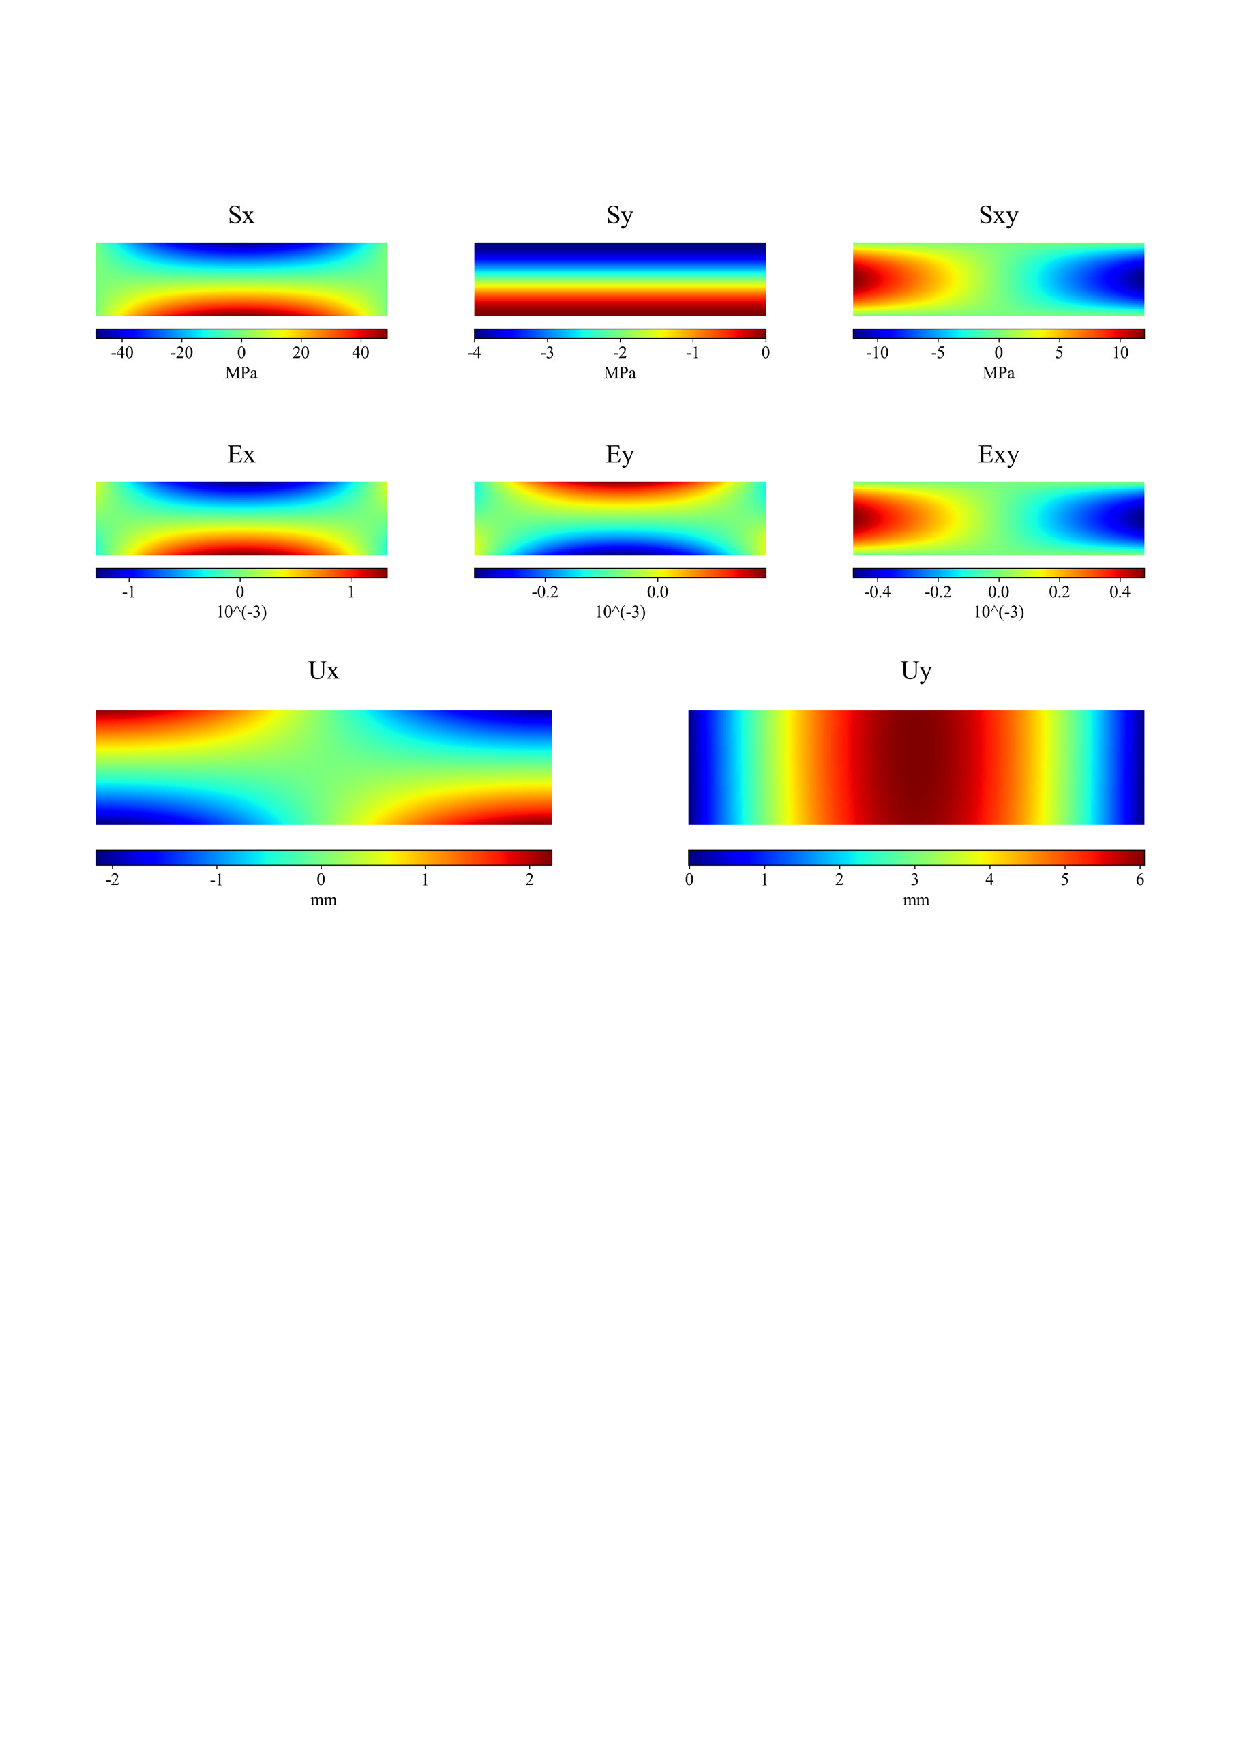
\includegraphics[width=1\textwidth]{figure2}
    \caption{计算结果云图}
    \label{fig:EPMplot}
\end{figure}
\subsection{结果讨论}
\label{cha:discussion1}
本章节,我们将简支梁当作平面应力问题来处理,且假设挤压应力~$\sigma_y$~沿~$x$~方向均匀分布。由于物体厚度方向尺寸较小,且受到的外力和约束只在梁的上下左右四个面,在前后面无约束。所以认为是平面应力问题是精确的。从结果来看,应力分量满足平衡微分方程、相容方程与边界条件,说明对挤压应力~$\sigma_y$~函数形式的假设这种是正确的。两端由于是小边界,即便不严格满足边界条件,对离两边较远处的应力也无影响。

实际问题中,梁厚度方向的尺寸不能满足平面应力问题的条件,且受到的外力和约束会更加复杂。以此为前提,想要得到解析解是十分困难的,因此,借助数值方法对实际问题进行求解得到的结果会对实际工程更有帮助。